\chapter{Resultados y Discusiones}
% [En este capítulo se presentan los resultados obtenidos correspondientes al proyecto descrito en el capítulo anterior. Los resultados se pueden presentar en tablas o gráfica y deben ser redactados y organizados de tal manera que sea fácil de comprender por los lectores.

% La los resultados no se explican por si mismo, por lo que es necesario una discusión que los explique y muestre cómo ayudan a resolver el problema definido en el capítulo 1. La discusión puede mencionar someramente los resultados antes de discutirlos, pero no debe repetirlos en detalle. No prolongues la discusión citando trabajos ``relacionados'' o planteando explicaciones poco probables. Ambas acciones distraen al lector y lo alejan de la discusión realmente importante. La discusión puede incluir recomendaciones y sugerencias para investigaciones futuras, tales como métodos alternos que podrían dar mejores resultados, tareas que no se hicieron y que en retrospectiva debieron hacerse, y aspectos que merecen explorarse en las próximas investigaciones.]
%! Vaciar los datos,

Durante la fase de evaluación del sistema, se estuvo recolectando información de las diversas estaciones meteorológicas instaladas en la región. Esta información permitió evaluar la viabilidad del proyecto a corto y mediano plazo, además, también facilitó realizar un análisis preeliminar de los datos recolectados. En la primer sección de este capítulo, se analizarán los datos recolectados por el sistema, posteriormente, se hará un análisis de la capacidad de extensibilidad del sistema para cubrir nuevos casos de uso y se terminará en pruebas de estrés y carga realizadas al mismo.

\section{Sobre los datos obtenidos}

Gracias a la información recabada durante el periodo de evaluación del sistema, fue posible realizar un análisis preeliminar de los datos recolectados de las estaciones. Dentro de estos datos se encuentra los tipos de incidencias, su duración y la fecha en la que éstas ocurrieron, así como, datos diversos específicos por cada tipo de incidencia.

Al revisar la información recolectada, se encontró que el mayor problema que se presenta en las estaciones es la inaccesibilidad por red a las mismas, como puede observarse en la figura \ref{fig:station-errors-by-type}. Esta falta de comunicación con las estaciones puede deberse a una serie de factores, como una conexión deficiente de red, problemas temporales del servicio de VPN con el que cuentan las estaciones, o la falta de energía en el dispositivo.

\begin{figure}[!ht]
   \centering
   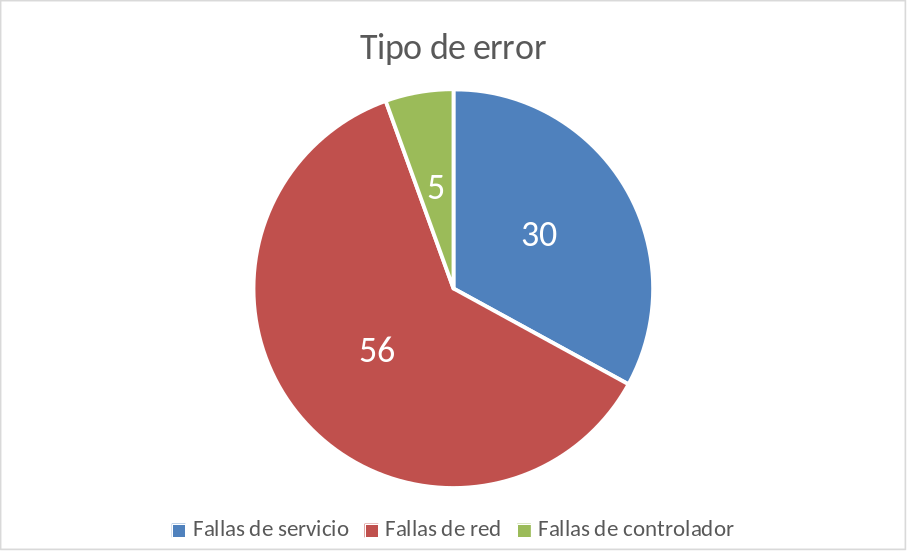
\includegraphics[width=0.7\linewidth]{images/graphs/by_type.png}
   \caption{Tipos de incidencia.}
   \label{fig:station-errors-by-type}
\end{figure}

Como se muestra en la Figura \ref{fig:station-incidents}, el número de incidentes es dependiente de cada estación, esto implica que no existe una coorelación entre ellas. Además, al compararlo con los datos obtenidos de la Figura \ref{fig:cumulated-downtime}, es posible observar que el número de fallas de red es directamente proporcional al tiempo de indisponibilidad de cada estación.

\begin{figure}[!ht]
   \centering
   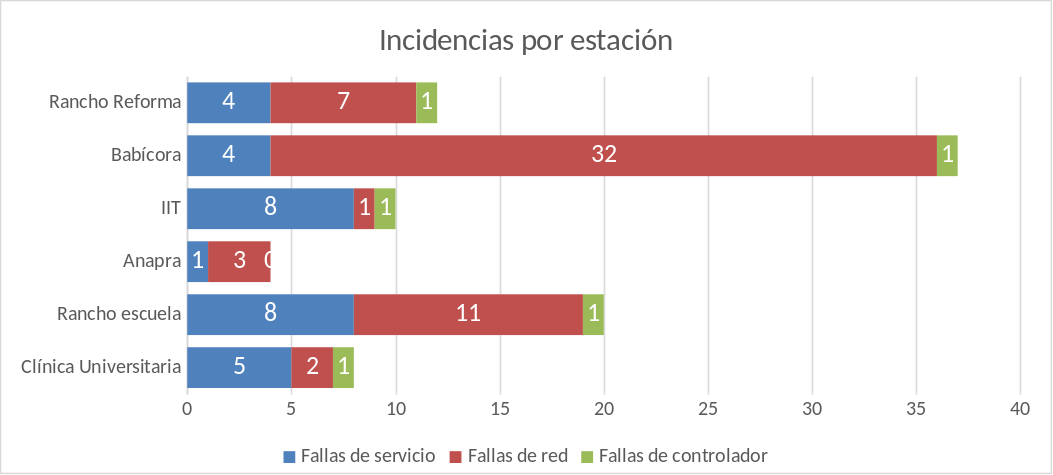
\includegraphics[width=0.9\linewidth]{images/graphs/by_station_incidents.png}
   \caption{Incidencias y sus tipos, agrupadas por estación.}
   \label{fig:station-incidents}
\end{figure}

\begin{figure}[!ht]
   \centering
   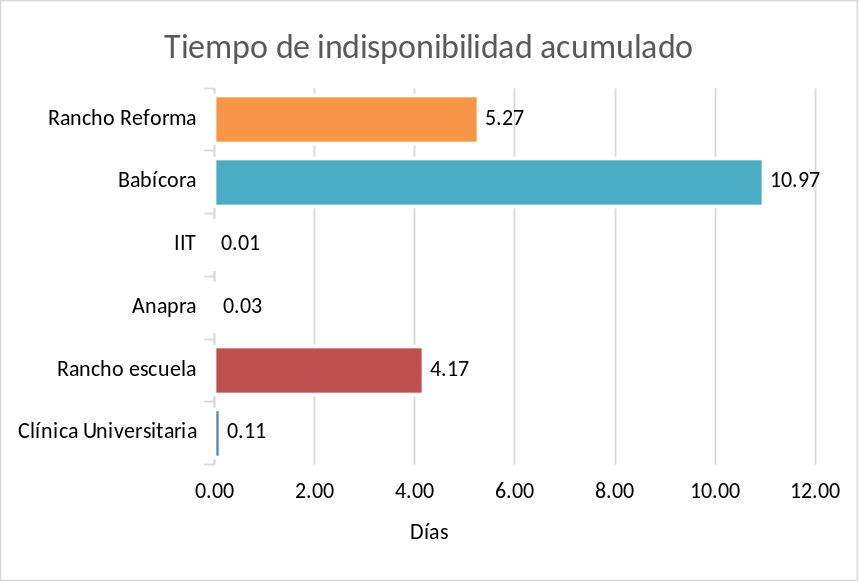
\includegraphics[width=0.65\linewidth]{images/graphs/cumulated_downtime.png}
   \caption{Tiempo de inaccesibilidad acumulado por estación.}
   \label{fig:cumulated-downtime}
\end{figure}

También, es posible observar que la falla que permaneció activa por más tiempo es un error en la base de datos MySQL que impedía el correcto almacenamiento de la información recabada por la estación. La pérdida de estos datos se puede verificar en la página de monitoreo de los datos generados de la estación en la Figura \ref{fig:rancho-data-loss} en la forma de ausencia de información en gráfica de la vista semanal de los sensores.

\begin{figure}[!ht]
   \centering
   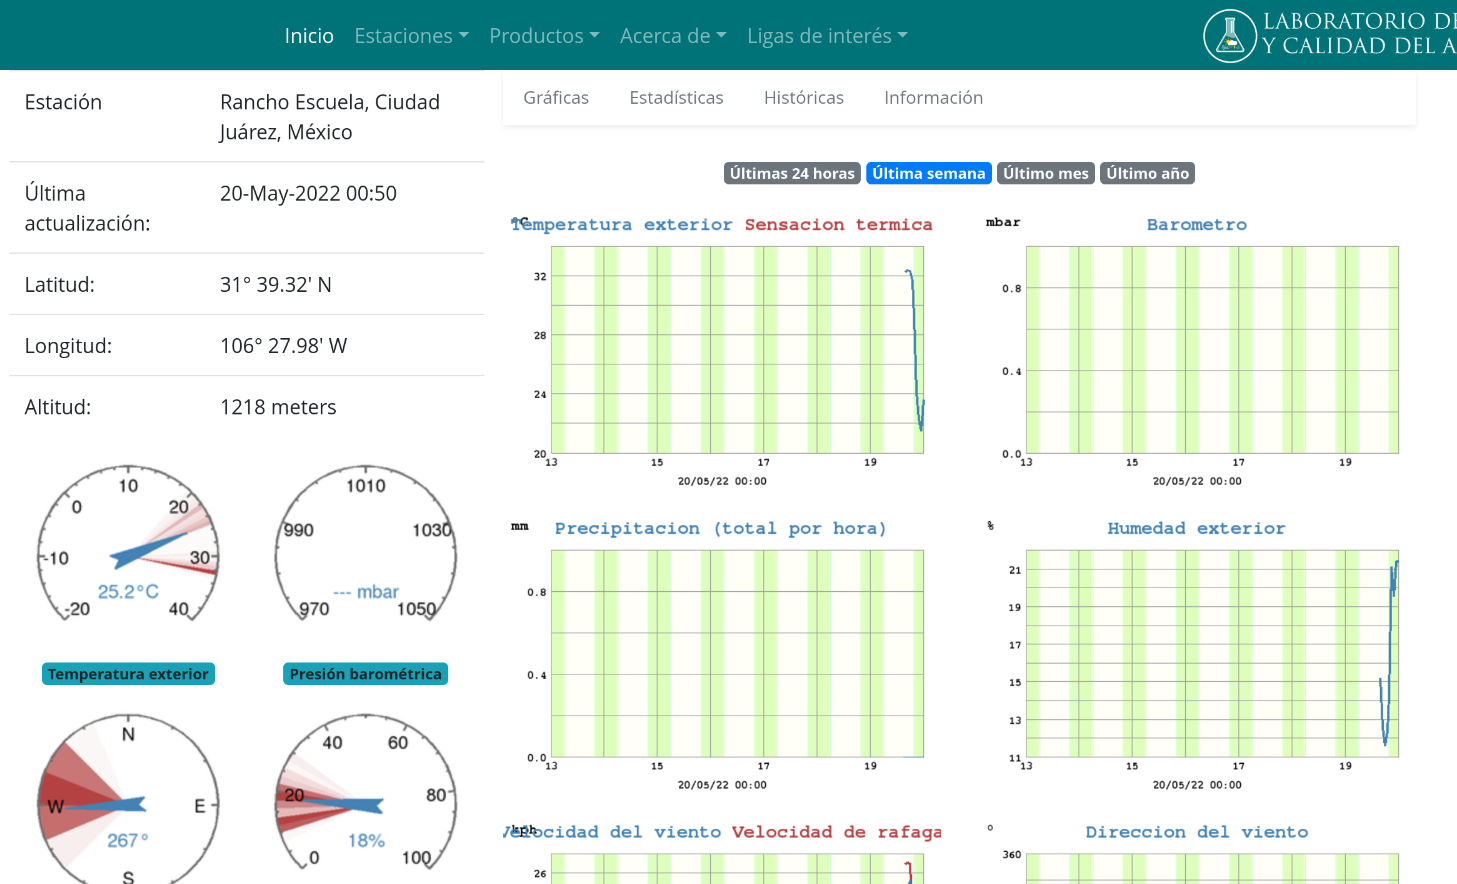
\includegraphics[width=1\linewidth]{images/screenshots/rancho-data-loss.png}
   \caption{Rancho escuela.}
   \label{fig:rancho-data-loss}
\end{figure}

El error de recolección de la información fue resuelto y la fecha de solución, como se muestra en la Figura \ref{fig:rancho-data-solved}, coincide con la pérdida de datos de la estación. Esto permite realizar una relación entre una falla concreta de una estación con la pérdida de información. Dicha información, puede ayudar al personal de CECATEV a realizar un proceso de mejora contínua para la evaluación y categorización de fallas de las estaciones, con el objetivo de priorizar los fallos que afectan la calidad de los datos como tarea primordial.

\begin{figure}[!ht]
   \centering
   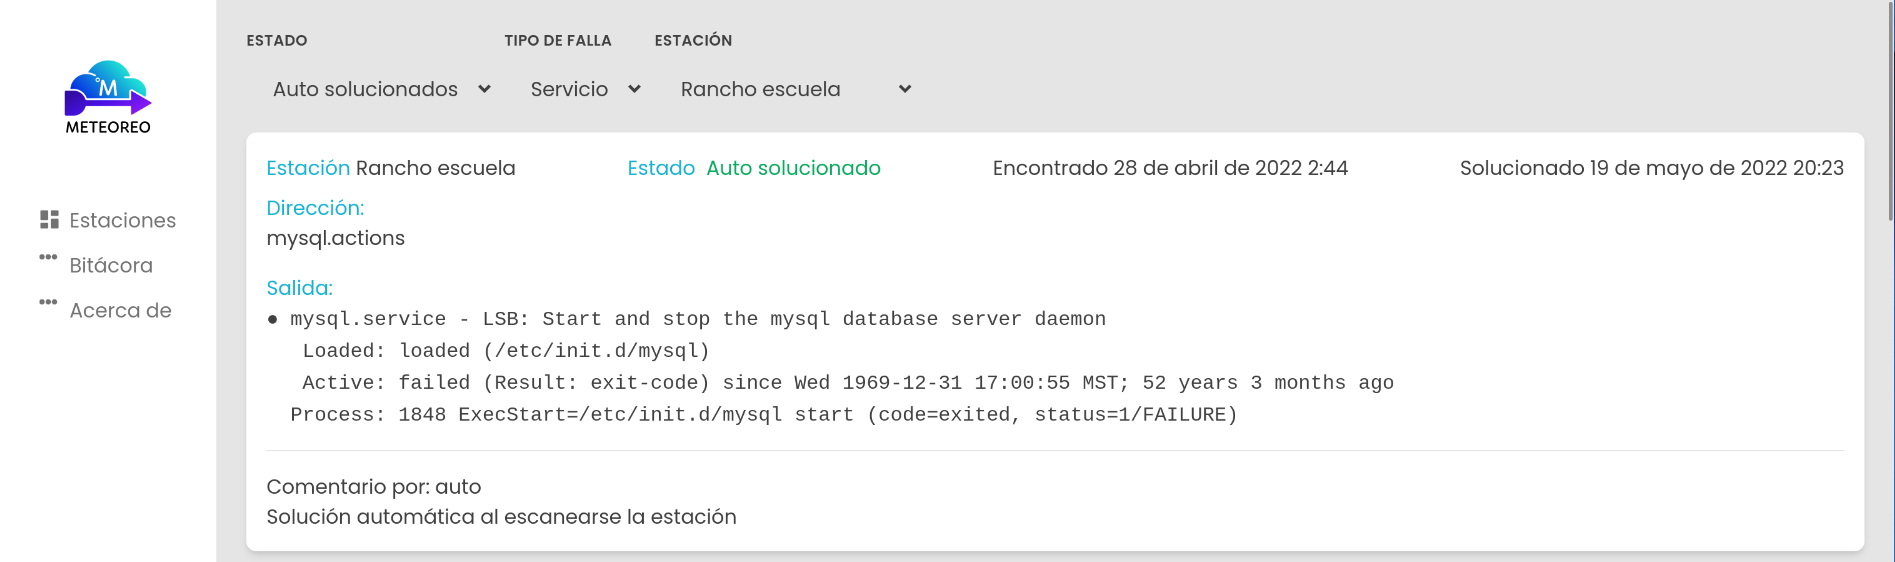
\includegraphics[width=1\linewidth]{images/screenshots/rancho-mysql-solved.png}
   \caption{Datos de falla de Rancho Escuela.}
   \label{fig:rancho-data-solved}
\end{figure}

% El proyecto finalizado, se compone de una cantidad aproximada de 3700 líneas de código, como se puede observar en el análisis de la herramienta \texttt{cloc} en la Figura \ref{fig:cloc}. Este proyecto se compone principalmente de componentes en Vue y scripts de Python.

% \begin{figure}[!ht]
%    \centering
%    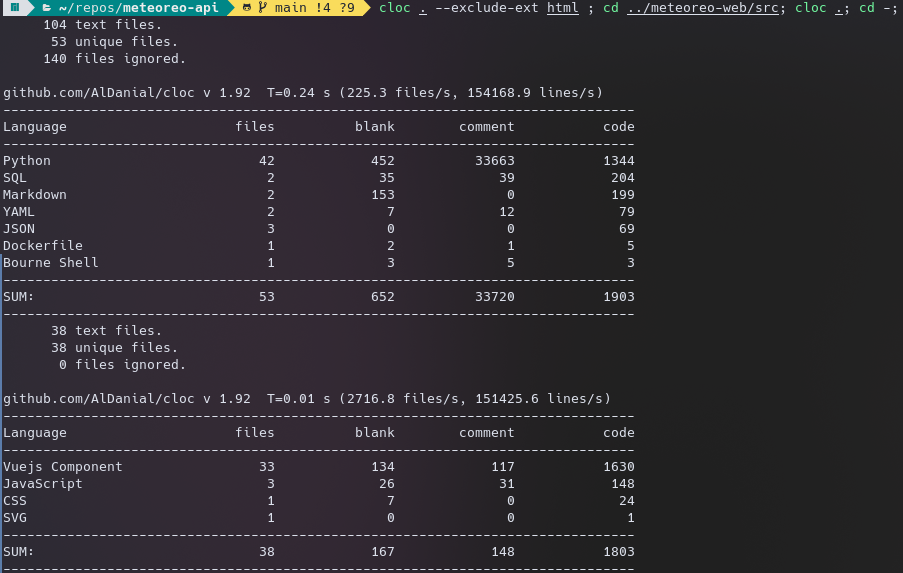
\includegraphics[width=0.8\linewidth]{images/screenshots/cloc}
%    \caption{Conteo de líneas de código.}
%    \label{fig:cloc}
% \end{figure}

\section{Sobre la extensibilidad del proyecto}

La modularidad del sistema y la forma en la que fue construído permite extenderlo, para que crear nuevos servicios sea una tarea trivial. Ésto, es gracias a que al ser una interfaz para ejecución de comandos, permite que las complejidades de monitoreo sean resueltas una sola vez, en la terminal de ejecución y siendo limitado sólo por la dificultad de la tarea que se busca llevar a cabo. Esto se puede ejemplificar creando un nuevo servicio de monitoreo y analizando la complejidad y el tiempo que llevan implementarlo.

Para este ejercicio, se seleccionó la tarea de crear un nuevo servicio para el monitoreo de uso de disco en las estaciones meteorológicas. Esto es importante, ya que aunque poseen un sistema de sólo lectura para asegurar la longevidad de las tarjetas SD, también cuentan con un sistema de respaldos local en memorias USB. El llevar este servicio de su concepción a un monitoreo activo, tomó aproximadamente 11 minutos, la adición de 16 líneas de código y la modificación de 2 como es posible ver en el Listado \ref{lst:git-diff-disk}. Si bien, fue una tarea sencilla haciendo uso de las amplias herramientas que poseen los sistemas en los que depende, también es importante notar que el sistema de monitoreo no agregó una fricción considerable para implementarlo.

\begin{listing}
\begin{minted}[%
   breaklines
]{diff}
diff --git a/app/lib/drivers/campbell.py b/app/lib/drivers/campbell.py
-from ..services import mysql, ropi, time, weewx, proxy, campbell
+from ..services import mysql, ropi, time, weewx, proxy, campbell, disk
[...]
+    "disk": disk.service,
[...]
diff --git a/app/lib/drivers/davis.py b/app/lib/drivers/davis.py
-from ..services import mysql, ropi, time, weewx
+from ..services import mysql, ropi, time, weewx, disk
[...]
+    "disk": disk.service,
[...]
diff --git a/app/lib/services/disk.py b/app/lib/services/disk.py
+service = {
+    "command": "PERCENT=$(df /mnt/usb --output=pcent | tail -n 1 | tr -d '%')" + \
+      "if (( $PERCENT > 80 )); then echo \"true $PERCENT\"; else echo \"false $PERCENT\"; fi",
+    "stdout": "false",
+    "stderr": None,
+    "actions": {
+        "disk_almost_full": {
+            "description": "El disco está casi lleno",
+            "solution": "Elimine algunos archivos de la estación",
+            "response_stdout": "true",
+            "response_stderr": None,
+        }
+    }
+}
\end{minted}
\caption{Diferencia de código al agregar el monitoreo de disco.}
\label{lst:git-diff-disk}
\end{listing}

\section{Sobre las capacidades de carga del proyecto}

Con la ayuda de la herramienta \href{https://locust.io/}{Locust}, se realizó una prueba de estrés y carga al sistema. Esta prueba se configuró para realizar pruebas en el sistema final en el que se realizó despliegue, la prueba se compone de dos rutas a probar (véase Listado \ref{lst:locust-config}), a las cuales se les realizarán peticiones con una cantidad creciente de usuarios concurrentes. Después de haber instalado la librería, se realizaron las pruebas con el comando \texttt{locust -H http://148.210.21.98:81 -u 50 -r 0.1 -t 300s --autostart}.

Al analisar la gráfica resultante, la Figura \ref{fig:locust-graphs}, de las pruebas, es posible observar que el tiempo de respuesta incrementa de forma lineal conforme a la cantidad de usuarios, comenzando con menos de 1 segundo por respuesta e incrementando hasta alcanzar casi 50 segundos por respuesta al tener a 50 usuarios concurrentes.

\begin{listing}
\begin{minted}[%
   breaklines
]{python3}
from locust import HttpUser, task

class API(HttpUser):
    @task
    def get_drivers(self):
        self.client.get("/api/v1/drivers/")

    @task
    def get_stations(self):
        self.client.get("/api/v1/stations/",  auth=("admin", "pass"))
\end{minted}
\caption{\texttt{lcoustfile.py} configuración de pruebas.}
\label{lst:locust-config}
\end{listing}


\begin{figure}[!ht]
   \centering
   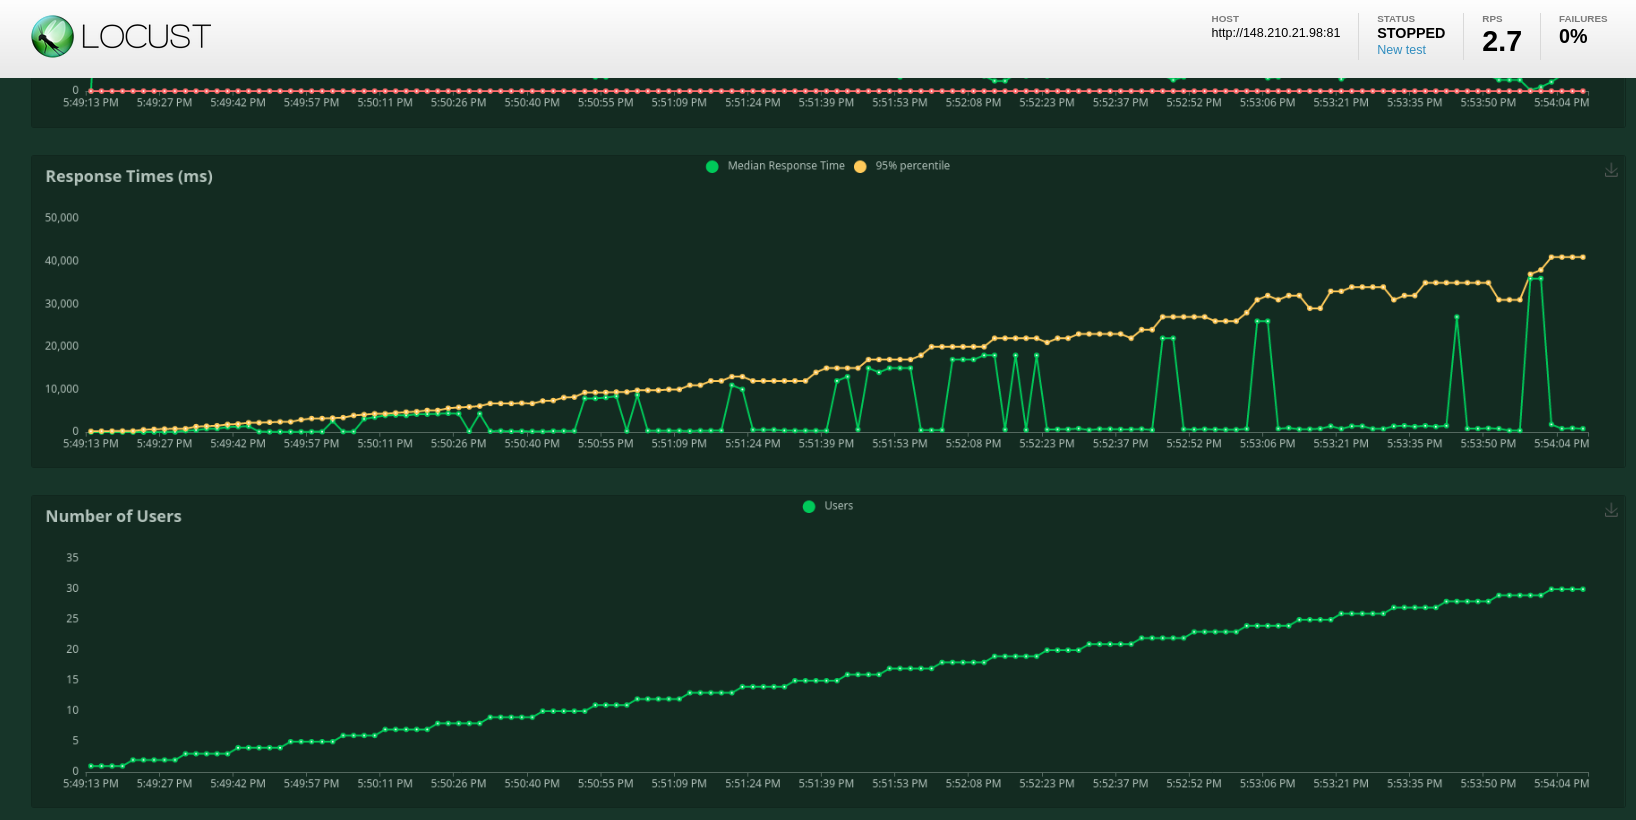
\includegraphics[width=1\linewidth]{images/screenshots/locust_graphs.png}
   \caption{Gráfica de usuarios y tiempos de respuesta creada con Locust.}
   \label{fig:locust-graphs}
\end{figure}

Sin embargo, al revisar el análisis de tiempo de respuesta por ruta presente en la Figura \ref{fig:locust-analysis}, es posible observar una diferencia significativa entre el tiempo de respuesta de la ruta \texttt{/api/v1/drivers}, con un máximo de 1.825s y la ruta \texttt{/api/v1/stations} con un máximo de 41.937s. Esto puede deberse a que la primer ruta mencionada no realiza tareas de lectura en la base de datos. Esto implicaría que la solución implementada para el almacenamiento de datos, una base de datos MariaDB en Docker en la misma máquina virtual que donde está alojado el API, no es una solución óptima para el problema.

\begin{figure}[!ht]
   \centering
   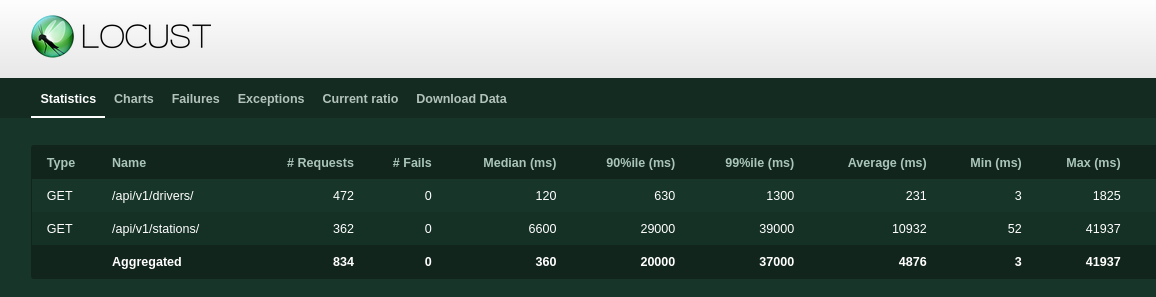
\includegraphics[width=1\linewidth]{images/screenshots/locust_analysis.png}
   \caption{Estadísticas de pruebas por ruta.}
   \label{fig:locust-analysis}
\end{figure}
